% Options for packages loaded elsewhere
\PassOptionsToPackage{unicode}{hyperref}
\PassOptionsToPackage{hyphens}{url}
%
\documentclass[
]{article}
\usepackage{lmodern}
\usepackage{amssymb,amsmath}
\usepackage{ifxetex,ifluatex}
\ifnum 0\ifxetex 1\fi\ifluatex 1\fi=0 % if pdftex
  \usepackage[T1]{fontenc}
  \usepackage[utf8]{inputenc}
  \usepackage{textcomp} % provide euro and other symbols
\else % if luatex or xetex
  \usepackage{unicode-math}
  \defaultfontfeatures{Scale=MatchLowercase}
  \defaultfontfeatures[\rmfamily]{Ligatures=TeX,Scale=1}
\fi
% Use upquote if available, for straight quotes in verbatim environments
\IfFileExists{upquote.sty}{\usepackage{upquote}}{}
\IfFileExists{microtype.sty}{% use microtype if available
  \usepackage[]{microtype}
  \UseMicrotypeSet[protrusion]{basicmath} % disable protrusion for tt fonts
}{}
\makeatletter
\@ifundefined{KOMAClassName}{% if non-KOMA class
  \IfFileExists{parskip.sty}{%
    \usepackage{parskip}
  }{% else
    \setlength{\parindent}{0pt}
    \setlength{\parskip}{6pt plus 2pt minus 1pt}}
}{% if KOMA class
  \KOMAoptions{parskip=half}}
\makeatother
\usepackage{xcolor}
\IfFileExists{xurl.sty}{\usepackage{xurl}}{} % add URL line breaks if available
\IfFileExists{bookmark.sty}{\usepackage{bookmark}}{\usepackage{hyperref}}
\hypersetup{
  pdftitle={CS5200 Fall 2020: Practicum 1},
  pdfauthor={Chandra Davis, Evan Douglass},
  hidelinks,
  pdfcreator={LaTeX via pandoc}}
\urlstyle{same} % disable monospaced font for URLs
\usepackage[margin=1in]{geometry}
\usepackage{graphicx,grffile}
\makeatletter
\def\maxwidth{\ifdim\Gin@nat@width>\linewidth\linewidth\else\Gin@nat@width\fi}
\def\maxheight{\ifdim\Gin@nat@height>\textheight\textheight\else\Gin@nat@height\fi}
\makeatother
% Scale images if necessary, so that they will not overflow the page
% margins by default, and it is still possible to overwrite the defaults
% using explicit options in \includegraphics[width, height, ...]{}
\setkeys{Gin}{width=\maxwidth,height=\maxheight,keepaspectratio}
% Set default figure placement to htbp
\makeatletter
\def\fps@figure{htbp}
\makeatother
\setlength{\emergencystretch}{3em} % prevent overfull lines
\providecommand{\tightlist}{%
  \setlength{\itemsep}{0pt}\setlength{\parskip}{0pt}}
\setcounter{secnumdepth}{-\maxdimen} % remove section numbering

\title{CS5200 Fall 2020: Practicum 1}
\author{Chandra Davis, Evan Douglass}
\date{}

\begin{document}
\maketitle

The steps we completed for Practicum 1 are detailed below. Please note
that there are links to each image that requires it in each section. We
decided to focus our attention on the case management aspect of the
contract tracing problem.

\hypertarget{conceptual-model-uml}{%
\subsection{Conceptual Model: UML}\label{conceptual-model-uml}}

View the conceptual model in Lucid Chart here:

\url{https://app.lucidchart.com/invitations/accept/5602312e-dfc3-4423-975c-47190ce6022e}

\includegraphics{imgs/CS5200 - Practicum 1_UML.png}\\

\hypertarget{logical-model-erd}{%
\subsection{Logical Model: ERD}\label{logical-model-erd}}

View the logical model in Lucid Chart here:

\url{https://app.lucidchart.com/invitations/accept/7b497cbf-268d-4a03-b1a7-822b5a844fea}

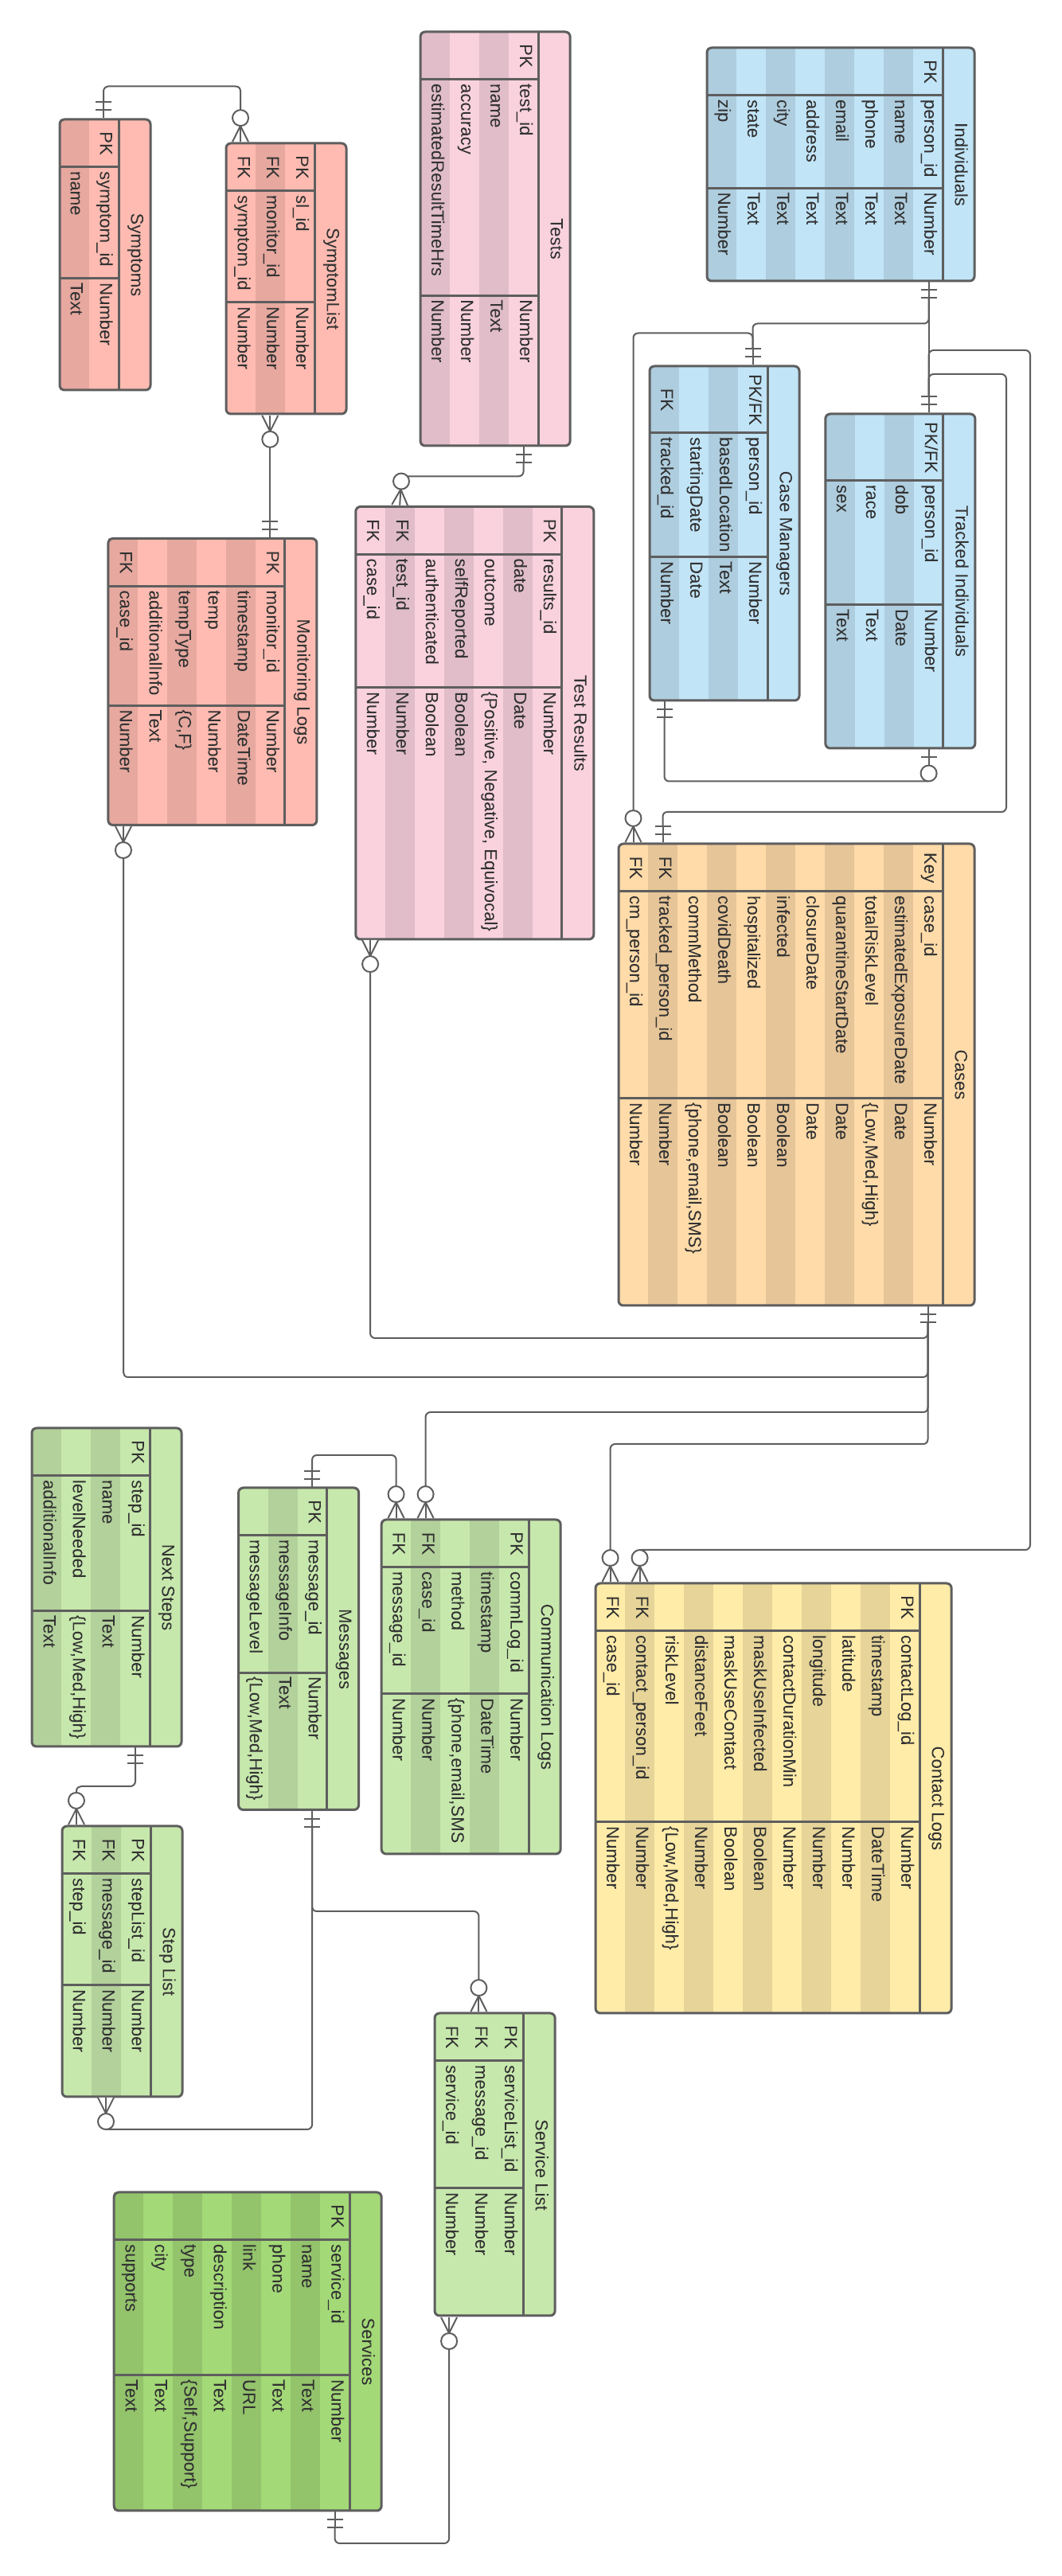
\includegraphics{imgs/CS5200 - Practicum 1_ERD.png}\\

\hypertarget{schema}{%
\subsection{Schema}\label{schema}}

View the schema in Google Docs here:

\url{https://docs.google.com/document/d/1o8pk51aed3BJSaBcwO2EMbT8I3ru_wpGTcTN4W-DbIM/edit?usp=sharing}

\includegraphics{imgs/Practicum1-Schema.png}\\

\hypertarget{creating-database-tables}{%
\subsection{Creating Database Tables}\label{creating-database-tables}}

Should you wish to inspect the scripts that create the database and
populate data, they can be found at:

\url{https://github.com/eldss-classwork/databases-practicum1-scripts}

The following images will show a progression from an empty database
through table creation in MySQL Workbench.

The MySQL Workbench start screen.

\includegraphics{imgs/MySQLWorkbench-IntroScreen.png}\\

The newly created, empty \texttt{test} database.

\includegraphics{imgs/MySQLWorkbench-emptydb.png}\\

The \texttt{test} database after table creation.

\includegraphics{imgs/MySQLWorkbench-create.png}\\

The following photos provide a detailed look at the schema of each table
as it was created in MySQL.

\includegraphics{imgs/Describe_CaseManagers.png}\\
\includegraphics{imgs/Describe_Cases.png}\\
\includegraphics{imgs/Describe_CommunicationLogs.png}\\
\includegraphics{imgs/Describe_CommMethods.png}\\
\includegraphics{imgs/Describe_ContactLogs.png}\\
\includegraphics{imgs/Describe_Individuals.png}\\
\includegraphics{imgs/Describe_Messages.png}\\
\includegraphics{imgs/Describe_MonitoringLogs.png}\\
\includegraphics{imgs/Describe_NextSteps.png}\\
\includegraphics{imgs/Describe_PossTestOutcomes.png}\\
\includegraphics{imgs/Describe_RiskLevels.png}\\
\includegraphics{imgs/Describe_ServiceList.png}\\
\includegraphics{imgs/Describe_Services.png}\\
\includegraphics{imgs/Describe_StepList.png}\\
\includegraphics{imgs/Describe_SymptomList.png}\\
\includegraphics{imgs/Describe_Symptoms.png}\\
\includegraphics{imgs/Describe_TestResults.png}\\
\includegraphics{imgs/Describe_Tests.png}\\
\includegraphics{imgs/Describe_TrackedIndividuals.png}\\

\hypertarget{populating-the-database}{%
\subsection{Populating The Database}\label{populating-the-database}}

The script for populating data into our database can be found at the
following link:

\url{https://github.com/eldss-classwork/databases-practicum1-scripts/blob/master/populate.sql}

Demonstrations that the data was loaded correctly can be found in the
queries below. That is, they return the data that was loaded.

\hypertarget{queries}{%
\subsection{Queries}\label{queries}}

\includegraphics{imgs/Query_Evan1.png}\\
\includegraphics{imgs/Query_Evan2.png}\\
\includegraphics{imgs/Query_Evan3.png}\\
\includegraphics{imgs/Query_Evan4.png}\\

\end{document}
